%%%%%%%%%%%%%%%%%%%%%%%%%%%%%%%%%%%%%%%%%
% Class Notes Template
% LaTeX Template
% By: Ryan Grove
%%%%%%%%%%%%%%%%%%%%%%%%%%%%%%%%%%%%%%%%%

%----------------------------------------------------------------------------------------
%	PACKAGES AND OTHER DOCUMENT CONFIGURATIONS
%----------------------------------------------------------------------------------------

\documentclass[paper=a4, fontsize=11pt]{scrartcl} % A4 paper and 11pt font size

\usepackage[T1]{fontenc} % Use 8-bit encoding that has 256 glyphs
\usepackage{fourier} % Use the Adobe Utopia font for the document - comment this line to return to the LaTeX default
\usepackage[english]{babel} % English language/hyphenation
\usepackage{amsmath,amsfonts,amsthm} % Math packages

\usepackage{lipsum} % Used for inserting dummy 'Lorem ipsum' text into the template

\usepackage{sectsty} % Allows customizing section commands
\allsectionsfont{\centering \normalfont\scshape} % Make all sections centered, the default font and small caps

\usepackage{fancyhdr} % Custom headers and footers
\pagestyle{fancyplain} % Makes all pages in the document conform to the custom headers and footers
\fancyhead{} % No page header - if you want one, create it in the same way as the footers below
\fancyfoot[L]{} % Empty left footer
\fancyfoot[C]{} % Empty center footer
%\fancyfoot[R]{\thepage} % Page numbering for right footer
\renewcommand{\headrulewidth}{0pt} % Remove header underlines
\renewcommand{\footrulewidth}{0pt} % Remove footer underlines
\setlength{\headheight}{13.6pt} % Customize the height of the header

\numberwithin{equation}{section} % Number equations within sections (i.e. 1.1, 1.2, 2.1, 2.2 instead of 1, 2, 3, 4)
\numberwithin{figure}{section} % Number figures within sections (i.e. 1.1, 1.2, 2.1, 2.2 instead of 1, 2, 3, 4)
\numberwithin{table}{section} % Number tables within sections (i.e. 1.1, 1.2, 2.1, 2.2 instead of 1, 2, 3, 4)

\setlength\parindent{0pt} % Removes all indentation from paragraphs - comment this line for an assignment with lots of text

\usepackage{lastpage}
\usepackage{fancyhdr}
\cfoot{\thepage\ of \pageref{LastPage}}

\def\v{\hbox{$\mathbf v$}}
\def\w{\hbox{$\mathbf w$}}
\def\u{\hbox{$\mathbf u$}}
\def\x{\hbox{$\textbf{x}$}}
\def\z{\hbox{$\mathbf z$}}
\def\a{\hbox{$\mathbf a$}}
\def\b{\hbox{$\mathbf b$}}
\def\L{\hbox{$\mathcal L$}}
\def\C{\hbox{$\mathbb C$}}
\def\B{\hbox{$\mathcal B$}}
\def\R{\hbox{$\mathbb R$}}
\def\X{\hbox{$\underline X$}}
\def\Q{\hbox{$\mathbb Q$}}
\def\R{\hbox{$\mathbb R$}}
\def\N{\hbox{$\mathbb N$}}
\def\C{\hbox{$\mathbb C$}}
\def\0{\hbox{$\mathbf 0$}}
\def\Y{\hbox{$\underline Y$}}
\def\a{\hbox{$\mathbf a$}}
\def\u{\hbox{$\mathbf u$}}
\def\w{\hbox{$\mathbf w$}}
\def\y{\hbox{$\mathbf y$}}
\def\X{\hbox{$\underline X$}}
\def\dd{\hbox{$\partial $}}
\def\B{\hbox{$\mathcal B$}}
\def\F{\hbox{$\mathcal F$}}
\def\L{\hbox{$\mathcal L$}}
\def\M{\hbox{$\mathcal M$}}
\def\D{\hbox{$\mathscr {D}$}}
\def\RR{\hbox{$\mathscr{R}$}}
\def\I{\hbox{$\mathcal I$}}

\usepackage{amssymb}
%\theoremstyle{plain}
\usepackage[margin = .75in]{geometry}
\newtheorem{claim}{Claim}
\newtheorem{theorem}{Theorem}[section]
\newtheorem{lemma}[theorem]{Lemma}
\newtheorem{proposition}[theorem]{Proposition}
\newtheorem{corollary}[theorem]{Corollary}
\newtheorem{problem}[theorem]{Problem}
%\theoremstyle{definition}
\newtheorem{definition}[theorem]{Definition}
%\theoremstyle{remark}
\newtheorem{remark}[theorem]{Remark}
\newtheorem{remarks}[theorem]{Remarks}
\newtheorem{example}[theorem]{Example}
\newcommand{\ds}{\displaystyle}
\newcommand{\ZZ}{\mathbb{Z}}
\newcommand{\QQ}{\mathbb{Q}}
\newcommand{\e}{\varepsilon}
\newcommand{\bbf}{\textbf}
\newcommand{\p}{\parallel}
\usepackage{color}
\newcommand{\field}[1]{\mathbb{#1}}
\usepackage{amsmath}
\usepackage{amsthm}
\usepackage{amssymb}
\usepackage{mathrsfs}
\usepackage{cancel}
\usepackage{upgreek}
\usepackage{graphicx}
\usepackage{multirow}
\usepackage{setspace}
\usepackage{url}
\usepackage{subfigure}
\usepackage{enumerate}
\usepackage{cases}
\usepackage{mathrsfs}
\usepackage{rotating}

%----------------------------------------------------------------------------------------
%	TITLE SECTION
%----------------------------------------------------------------------------------------

\newcommand{\horrule}[1]{\rule{\linewidth}{#1}} % Create horizontal rule command with 1 argument of height

\title{	
\normalfont \normalsize 
\textsc{Ryan Grove, Clemson University, MATH1080 - 9} \\ [25pt] % Your name, university, class
\horrule{0.5pt} \\[0.4cm] % Thin top horizontal rule
\huge Section 10.3: Polar Coordinates  \\ % The assignment title
\horrule{2pt} \\[0.5cm] % Thick bottom horizontal rule
}

\author{Date:} % The due date

\date{\normalsize April 18, 2016} % A custom date

\begin{document}

\maketitle % Print the title

\begin{flushleft}
\begin{tabular}{l l}
Name: \rule{3.2in}{.01cm}  & {}%Table number: \rule{1in}{.01cm}\\
\end{tabular}
\end{flushleft}

%----------------------------------------------------------------------------------------
%	Lecture
%----------------------------------------------------------------------------------------

\section*{\textbf{Lecture:}}

A coordinate system represents a point in the plane by an ordered pair of numbers called coordinates. Usually we use Cartesian coordinates (x,y), which are directed distances from two perpendicular axes. In this section we describe a coordinate system introduced by Newton, called the \underline{\hspace{1in}} \underline{\hspace{1.25in}} \underline{\hspace{1in}}, which is more convenient for many purposes.\\
\indent

We choose a point in the plane that is called the \underline{\hspace{0.75in}} (or origin) and is labeled $O$. Then we draw a ray (half-line) starting at $O$ called the \underline{\hspace{1in}} \underline{\hspace{0.75in}}. This axis is usually drawn horizontally to the right and corresponds to the positive $x$-axis in the Cartesian coordinates.\\
\indent

If $P$ is any other point in the plane, let \underline{\hspace{0.3in}} be the distance from $O$ to $P$ and let \underline{\hspace{0.3in}} be the angle (usually measured in radians) between the polar axis and the line $OP$ as in Figure 1.
\[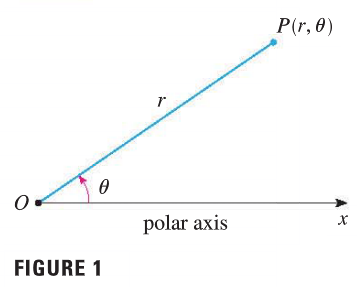
\includegraphics[scale=0.4]{10-3pic1.png} \quad \quad \quad 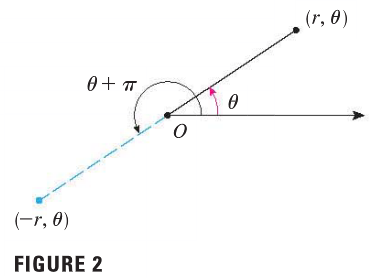
\includegraphics[scale=0.4]{10-3pic2}\]

Then the point $P$ is represented by the ordered pair \underline{\hspace{1in}} and $r,\theta$ are called the \underline{\hspace{1in}} \underline{\hspace{1.5in}} of $P$. We use the convention that an angle is positive if measured in the counterclockwise direction from the polar axis and negative in the clockwise direction. If $P=O$, then $r=0$ and we agree that $(0,\theta)$ represents the pole for any value of $\theta$.\\
\indent

We extend the meaning of polar coordinates $(r,\theta)$ to the case in which $r$ is negative by agreeing that, as in Figure 2 (above), the points $(-r,\theta)$ and $(r,\theta)$ lie on the same line through $O$ and at the same distance $|r|$ from $O$, but on opposite sides of $O$.
\begin{itemize}
\item If $r>0$, the point $(r,\theta)$ lies in the same quadrant as $\theta$; \\
\item If $r<0$, the point $(r,\theta)$ lies in the quadrant on the opposite side of the \textit{pole}.
\end{itemize}

*Notice that $(r,\theta)$ represents the same point as $(r,\theta + \pi)$.\\
\indent

\underline{Example 1}: Plot the points whose polar coordinates are given.
\[(a) \text{ } (1,\ds\frac{5\pi}{4}) \hspace{75pt} (b) \text{ } (2,3\pi) \hspace{75pt} (c) \text{ } (2,\ds\frac{-2\pi}{3}) \hspace{75pt} (d) \text{ } (-3,\ds\frac{3\pi}{4})\]
\indent

\vspace{2in}


\underline{Note}: In the Cartesian coordinate system every point has only one representation, but in the polar coordinate system each point has many representations. \\
\indent

For instance, the point $(1,\ds\frac{5\pi}{4})$ in Example 1(a) could be written as $(1,-\ds\frac{3\pi}{4})$, $(1,\ds\frac{13\pi}{4})$, or $(-1,\ds\frac{\pi}{4})$. 

\[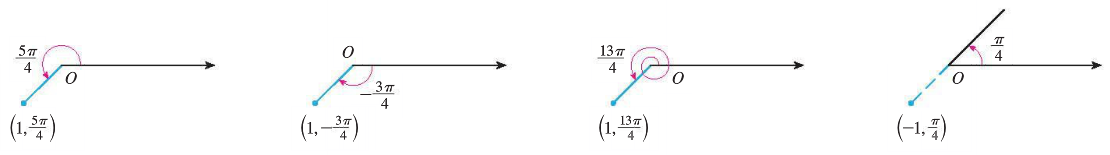
\includegraphics[scale=0.45]{10-3pic4.png}\]

In fact, since a complete counterclockwise rotation is given by an angle $2\pi$, the point represented by polar coordinates $(r,\theta)$ is also represented by 
\[(r,\theta + 2n\pi) \quad \text{ and } \quad (-r,\theta + (2n+1)\pi)\]

where $n$ is any integer.\\
\indent

\section*{Connection between Polar and Cartesian Coordinates}

\[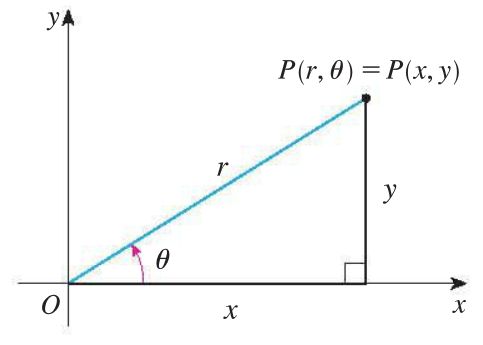
\includegraphics[scale=0.45]{10-3pic5.png}\]

If the point $P$ has Cartesian coordinates $(x,y)$ and polar coordinates $(r,\theta)$, then we have

\[\cos\theta = \ds\frac{x}{r} \quad \quad \sin\theta = \ds\frac{y}{r}\]


and so\\
\indent

\underline{Polar to Cartesian}:
\begin{equation}
\boxed{\text{ } x = r\cos\theta \quad \quad y = r\sin\theta \text{ }} \label{(1)}
\end{equation}

\underline{Cartesian to Polar}:
\begin{equation}
\boxed{\text{ } r^2 = x^2 + y^2 \quad \quad \tan\theta = \ds\frac{y}{x}\text{ }} \label{(2)}
\end{equation}
\indent

\vspace{.5in}
\underline{Example 2}: Convert the point $(2,\ds\frac{\pi}{3})$ from polar to Cartesian coordinates.\\
\indent

\vspace{1.75in}

\underline{Example 3}: Represent the point with Cartesian coordinates $(1,-1)$ in terms of polar coordinates.\\
\indent

\vspace{1.9in}

\underline{Note}: Equations 2 do not uniquely determine $\theta$ when $x$ and $y$ are given because, as $\theta$ increases through the interval $0\leq \theta < 2\pi$, each value of $\tan\theta$ occurs twice. Therefore, in converting from Cartesian to polar coordinates, it's not good enough to just find $r$ and $\theta$ that satisfy Equations 2. As in Example 3, we must choose $\theta$ so that the point $(r,\theta)$ lies in the correct quadrant.

\section*{Polar Curves}

The graph of a polar equation $r=f(\theta)$, or more generally $F(r,\theta) = 0$, consists of all points $P$ that have at least one polar representation $(r,\theta)$ whose coordinates satisfy the equation.\\
\indent

\underline{Example 4}: What curve is represented by the polar equation $r=2$?\\
\indent

\textbf{SOLUTION:} The curve consists of all points $(r,\theta)$ with $r=2$. Since $r$ represents the distance from the point to the pole, the curve $r=2$ represents the \underline{\hspace{1in}} with center $O$ and radius \underline{\hspace{0.3in}}. In general, the equation $r=a$ represents a circle with center $O$ and radius $|a|$.
\[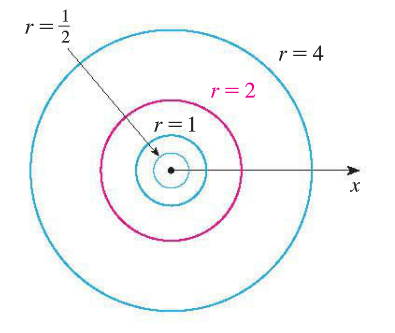
\includegraphics[scale=0.39]{10-3pic6.png}\]

\underline{Example 5}: Sketch the polar curve $\theta = 1$.\\
\indent

\vspace{2.5in}

\underline{Example 6}:
\begin{enumerate}
\item[(a)] Sketch the curve with polar equation $r=2\cos\theta$.\\
\item[(b)] Find a Cartesian equation for this curve.\\
\end{enumerate}
\indent

\vspace{5in}

\newpage
\underline{Example 7}: Sketch the curve $r=1+\sin\theta$.\\
\indent

\textbf{SOLUTION}: Instead of plotting points as in Example 6, we first sketch the graph of $r=1+\sin\theta$ in \textit{Cartesian} coordinates in Figure 10 by shifting the sine curve up one unit. This enables us to read at a glance the values of $r$ that correspond to increasing values of $\theta$.\\

\[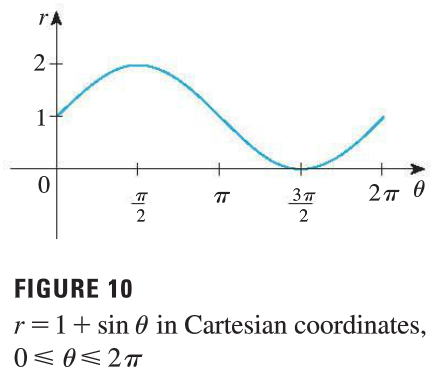
\includegraphics[scale=0.4]{10-3pic10.png}\]

\begin{itemize}
\item As $\theta$ increases from $0$ to $\ds\frac{\pi}{2}$, $r$ increases from 1 to 2 [Figure 11(a)]
\item As $\theta$ increases from $\ds\frac{\pi}{2}$, $r$ decreases from 2 to 1 [Figure 11(b)]
\item As $\theta$ increases from $\pi$ to $\ds\frac{3\pi}{2}$, $r$ decreases from 1 to 0 [Figure 11(c)]
\item As $\theta$ increases from $\ds\frac{3\pi}{2}$ to $2\pi$, $r$ increases from 0 to 1 [Figure 11(d)]
\end{itemize}

\underline{Note}: $\theta < 0$ or $\theta > 2\pi$ simply retraces the path represented by $0\leq \theta \leq 2\pi$.\\
\indent

Putting together the parts of the curve from Figure 11(a)-(d), we sketch the complete curve in part (e). It is called a \underline{\hspace{1.25in}} because it is shaped like a heart.\\

\[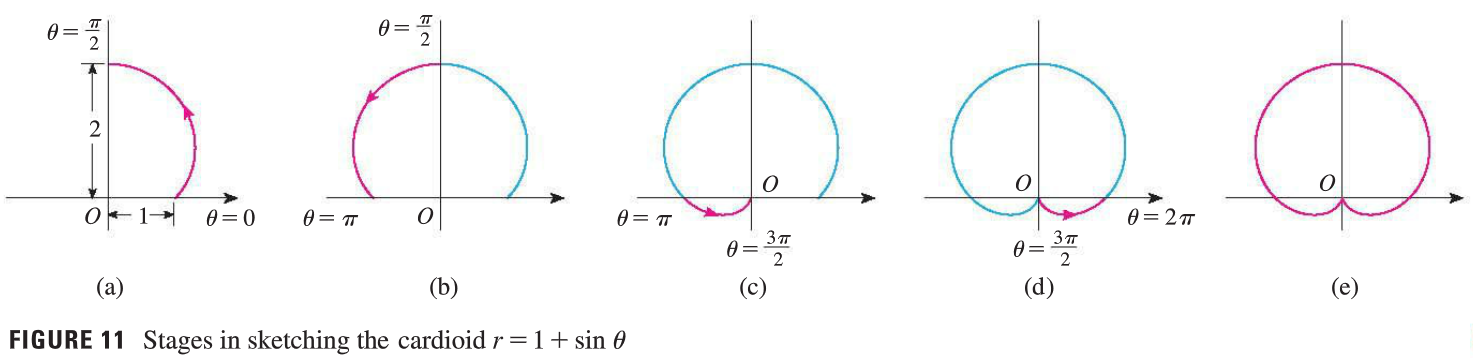
\includegraphics[scale=0.35]{10-3pic11.png}\]
\indent

\newpage
\underline{Example 8}: Sketch the curve $r=\cos 2\theta$.\\
\indent

\textbf{SOLUTION}: As in Example 7, we first sketch $r=\cos 2\theta$, $0\leq \theta \leq 2\pi$, in Cartesian coordinates in Figure 12.

\begin{itemize}
\item As $\theta$ increases from 0 to $\ds\frac{\pi}{4}$, $r$ decreases from 1 to 0 [Fig. 13 \textcircled{1}]
\item As $\theta$ increases from $\ds\frac{\pi}{4}$ to $\ds\frac{\pi}{2}$, $r$ goes from 0 to $-1$ [Fig. 13 \textcircled{2}]
\vdots
\end{itemize}

The resulting curve has four loops and is called a \underline{\hspace{1.5in}} \underline{\hspace{0.75in}}.
\[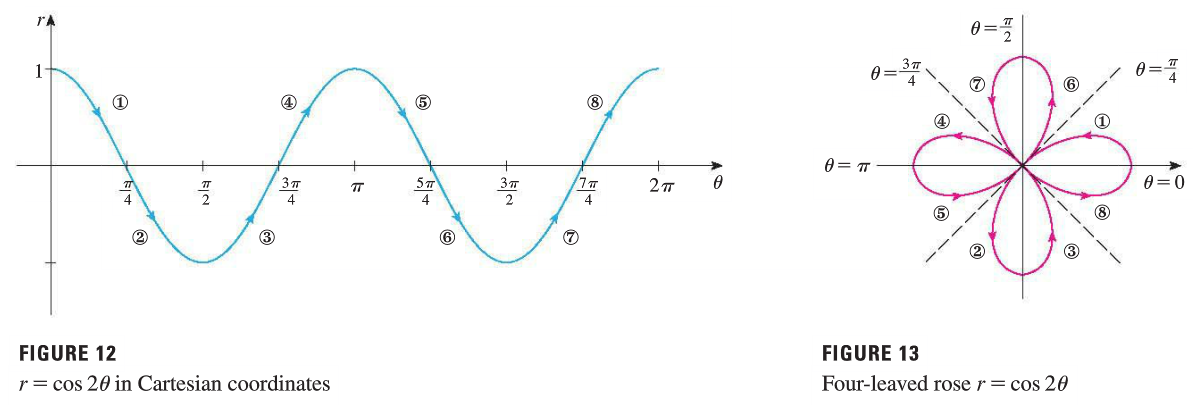
\includegraphics[scale=0.38]{10-3pic12.png}\]

\section*{Symmetry}

When we sketch polar curves it is sometimes helpful to take advantage of symmetry. The following three rules are explained in Figure 14.

\begin{enumerate}
\item[(a)] If a polar equation is unchanged when $\theta$ is replaced by $-\theta$, the curve is symmetric about the polar axis.
\item[(b)] If the equation is unchanged when $r$ is replaced by $-r$, or when $\theta$ is replaced by $\theta + \pi$, the curve is symmetric about the pole. (This means that the curve remains unchanged if we rotate it through $180^{\circ}$ about the origin.)
\item[(c)] If the equation is unchanged when $\theta$ is replaced by $\pi-\theta$, the curve is symmetric about the vertical line $\theta = \ds\frac{\pi}{2}$.
\end{enumerate}
\[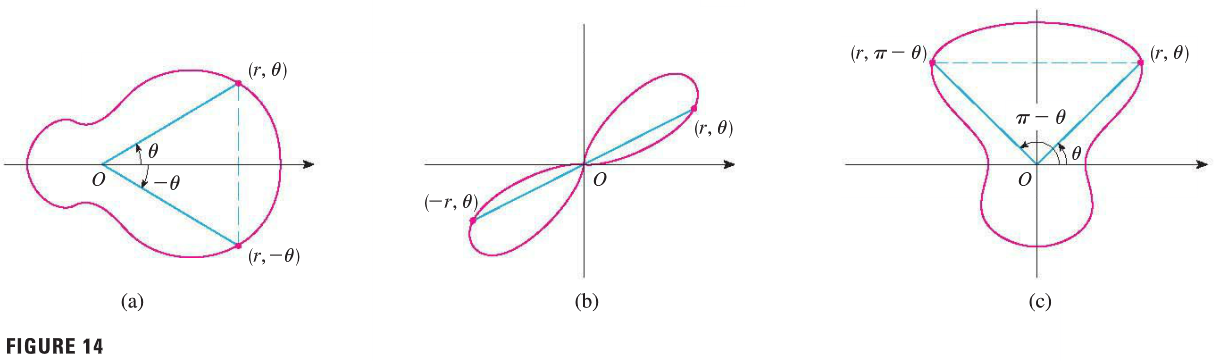
\includegraphics[scale=0.38]{10-3pic14.png}\]

\section*{Tangents to Polar Curves}
to find a tangent line to a polar curve $r=f(\theta)$, we regard $\theta$ as a parameter and write its parametric equation as
\vspace{-10pt}
\[x=r\cos\theta = f(\theta)\cos\theta \quad \quad y = r\sin\theta = f(\theta)\sin\theta\]
Then,
\vspace{-15pt}
\begin{equation}
\ds\frac{dy}{dx} = \ds\frac{\ds\frac{dy}{d\theta}}{\ds\frac{dx}{d\theta}} = \ds\frac{\ds\frac{dr}{d\theta}\sin\theta + r\cos\theta}{\ds\frac{dr}{d\theta}\cos\theta - r\sin\theta} \label{5}
\end{equation}
We locate...
\vspace{-10pt}
\begin{itemize}
\item \textbf{Horizontal tangents} by finding the points where $\ds\frac{dy}{dx} = 0$ (Either $\ds\frac{dy}{d\theta} = 0$ and $\ds\frac{dx}{d\theta}\neq 0$ or the limit of $\ds\frac{dy}{dx}=0$).
\vspace{-10pt}
\item \textbf{Vertical tangents} at the points where either $\ds\frac{dx}{d\theta}=0$ and $\ds\frac{dy}{d\theta}\neq 0$ or the limit of $\ds\frac{dy}{dx}=\pm\infty$.\\
\end{itemize}
\indent

\underline{Example 9}:
\begin{enumerate}
\item[(a)] For the cardioid $r=1+\sin\theta$ of Example 7, find the slope of the tangent line $\theta = \ds\frac{\pi}{3}$.\\
\end{enumerate}
\newpage
\underline{Example 9 continued...}
\begin{enumerate}
\item[(b)] Find the points on the cardioid where the tangent line is horizontal or vertical.
\end{enumerate}

\newpage

\[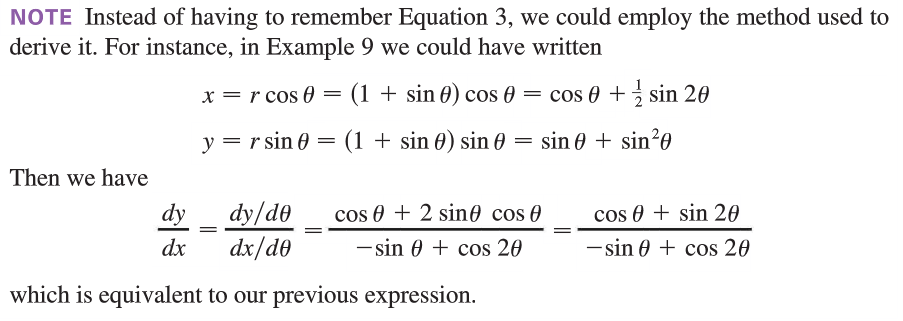
\includegraphics[scale=0.5]{10-3note.png}\]
\indent

\underline{Example 11}: Investigate the family of polar curves given by $r=1+c\sin\theta$. How does the shape change as $c$ changes? (These curves are called \underline{\hspace{1.25in}}, after a French word for snail, because of the shape of the curves for certain values of $c$.)\\
\indent

\textbf{SOLUTION}: Figure 19 shows computer-drawn graphs for various values of $c$.\\
\begin{itemize}
\item For $c>1$ there is a loop that decreases in size as $c$ decreases
\item When $c=1$ the loop disappears and the curve becomes the cardioid that we sketched in Example 7
\item For $\ds\frac{1}{2} \leq c < 1$ the cardioid's cusp is smoothed out and becomes a "dimple".
\item For $0\leq c \leq \ds\frac{1}{2}$, the limacon is shaped like an oval. This oval becomes more circular as $c\to 0$, and when $c=0$ the curve is just the circle $r=1$.
\end{itemize}

%----------------------------------------------------------------------------------------

\end{document}